\documentclass[conference]{sig-alternate-05-2015}

%\usepackage[active]{srcltx}
%\usepackage[pdftex]{graphicx} 
%\usepackage{savetrees}
%\usepackage{caption}

\usepackage[utf8x]{inputenc} 
\usepackage{comment}  \usepackage{graphicx} \usepackage{amsmath}        
\usepackage{varwidth} \usepackage{framed}    
\usepackage{paralist} \usepackage{lastpage} \usepackage{hyperref}
\usepackage{amsfonts} \usepackage{multicol} \usepackage{times}
\usepackage{mdwlist}  \usepackage{hyphenat} \usepackage{color}
\usepackage{array}    \usepackage{fancyhdr} \usepackage{booktabs}
\usepackage{floatrow}

\usepackage{tinycaptionfont} 

\usepackage{bibspacing} 
\setlength{\bibspacing}{2.0\baselineskip}

%\newcommand{\comments}[1]{}


\usepackage{fixltx2e}
\usepackage{hyperref}
\usepackage{url}


\begin{document}

\title{Phenomenologically Augmented Reality With New Wearable LED Sequential Wave Imprinting Machines}

\author{
\ACMauthorblockN{Pete Scourboutakos, Sarang Nerkar, Max Hao Lu, Steve Mann}\\
\ACMauthorblockA{Dept.\ of Electrical and Computer Engineering\\
University of Toronto\\ Toronto, Canada\\
{\footnotesize\texttt{\{pete, sarang, max, mann\}{@}eyetap.org}}}}
\maketitle


\begin{abstract}

The Sequential Wave Imprinting Machine (SWIM), invented by Steve Mann in the 1970s, offers an augmediated reality experience which a group of people can all see with the naked eye (i.e. without the need to wear any special eyeglass).\\
The SWIM is waved back-and-forth in space, and, through persistence of exposure (to either human sight, or to a camera such as by way of photographic film or sensor array) makes waves visible.  Unlike displaying waves on an oscilloscope, SWIM displays waves arranged in space in such a way that they are registered not only in real-time but also in real-space, providing a naturally augmented reality. \\
This paper outlines improvements in SWIM which are made possible by a simple circuit (with only 2 transistors per element), and recent improvements in LED technology.  The result makes possible greater resolution and more dense packing, making it more wearable, and thus more accessible in general. Photos and scientific results of the new SWIM are presented.\\
\end{abstract}

% For peer review papers, you can put extra information on the cover
% page as needed:
% \ifCLASSOPTIONpeerreview
% \begin{center} \bfseries EDICS Category: 3-BBND \end{center}
% \fi
%
% For peerreview papers, this IEEEtran command inserts a page break and
% creates the second title. It will be ignored for other modes.

\IEEEpeerreviewmaketitle


\section{Introduction}
Augmediated reality is an experience where by the means of a system of technology, people are able to seamlessly improve or otherwise alter their perception of reality, while situated in reality, which is real-time and real-space. \\
Where for reality dB = 1, augmediated reality systems may be organized into three types: \\

\begin{enumerate}
\item dB\textgreater  0 - Those of augmentation, which involve amplification / enhancement / addition of information, such as the system presented here. These systems are augmented reality.
\item dB\textless  0 - Those of diminishment which involve attenuation / subtraction of information, such as HDR for welding. ~\cite{mannHDR} These systems are diminished reality.
\item dB E R - Those which are dynamic and can do both, as needed.
\end{enumerate}

Many augmediated reality systems are of the third type, designed as a generalized platform with the intention of supporting a variety of applications, which is in line with the way most personal computers (including smartphones) are thought of as being interacted with ~\cite{arsurvey}. These systems consist of input and output devices, often cameras and aremacs respectively, with computer processing in between ~\cite{mann2012realtime}. Thanks to ongoing advancements in miniturization and wearable computer technology, there is large scale interest and commercial development ongoing in these areas ~\cite{mann1998wearable}. The challenge with a system of this complexity is for it to embody the principles of humanistic intelligence ~\cite{mann1998humanistic} which are key to a system which will provide a seamless and convincing experience which can advance technology for humanity.~\cite{mann2001wearable}\\
%What is more is that a high level of complexity 
The augmediated reality system in this paper is strictly additive (type 1). It is also purpose built for the specific application of the visualization of radio waves, in the same fashion as early augmediated reality experiments carried out by Steve Mann in the 1970s. ~\cite{mann2015phenomenal} Recently, with the availability of high efficiency and small SMD LEDs, the SWIM no longer relies on incandescent bulbs and has thus become more practical. \\
This paper presents two new incarnations of SWIM. The first is based on the LM3914 and provides high resolution (10pixels/cm) at the price of a larger board size. The second is a novel circuit which is used to make a small wearable SWIM which is unprecedented in volume, making these experiments in augmediated reality ever more practical as a wearable.\\
%LED technology has existed since the 1970s (60s?) but until the last decade remained only practical for low light applications of indication, due to a severe limitation in light output compared to other sources of light such as incandescants, or fluourescents. Recent advances in semiconductor device design for LEDs has made LEDs practical for applications of lighting and display beyond simple indication, as made apparant by the availablilty of LED televisions in (2009/2012 Sony).[wikipedia, how do we cite something like this? cite a product]\\
Head mounted displays, ~\cite{mann1997wearable} have been used extensively as the output device of choice for augmediated reality systems, ~\cite{caudell1992augmented}. This is natural because they are usually already designed to work as computer displays. These types of devices are well suited to personal augmediated reality experiences, but do not work as easily for activities where multiple people or groups of people are involved and wish to partake in the same experience. For everyone to participate, everyone must wear their own pair of glasses, and high level software/networking systems are required to render the experience for everyone. This creates bottleneck points and opens up opportunities for delays and other issues which can strip the system of its humanistic intelligence, making the experience anything from less convincing to illness inducing to painful. ~\cite{drascic1996perceptual} \begin{figure}
\centering
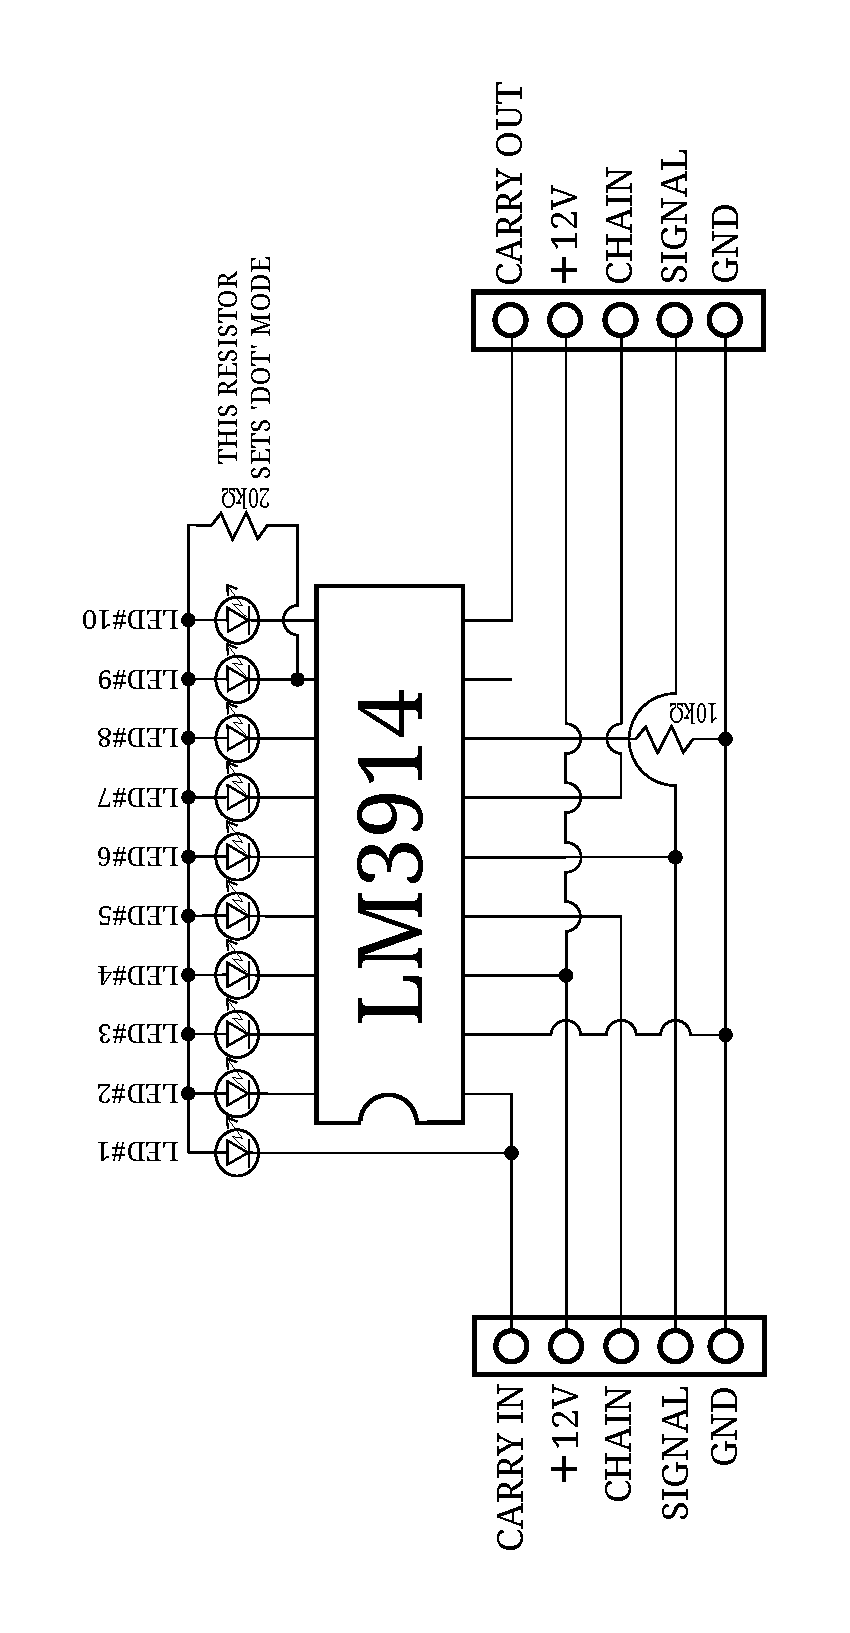
\includegraphics[scale = 0.274, angle = 270]{3914schem.pdf}
\caption{\label{fig:frog}Schematic of modular LM3914 SWIM device.}
\end{figure}
The SWIM system forfeits the complexity imposed by the need for a general purpose system, and instead focuses as a single-purpose-built augmediated reality system which makes visible normally invisible radio waves. In order to achieve this effect, the SWIM is simply driven with the doppler return output of any low power X band microwave radar set.
The SWIM works similarly to an oscilloscope with no timebase generator, by painting out a sensed/measured wave in light so that it is made visible. Instead of the effect of the oscilloscope phosphor we have the phenomenon of persistance of exposure ~\cite{mann2015phenomenal}. An oscilloscope works in real-time but virtual-space, on its own 2D display, like most AR systems, while the SWIM uses a 1D display to produce an image like a 2D holograph, which is registered in real-time as well as in real-space, as the user sweeps the SWIM device itself through the waves in space. 
Last and perhaps most importantly, the augmediated reality experience SWIM creates is easily shared among a group of people, all of whom may bear witness with the naked eye.
\begin{figure}
\centering
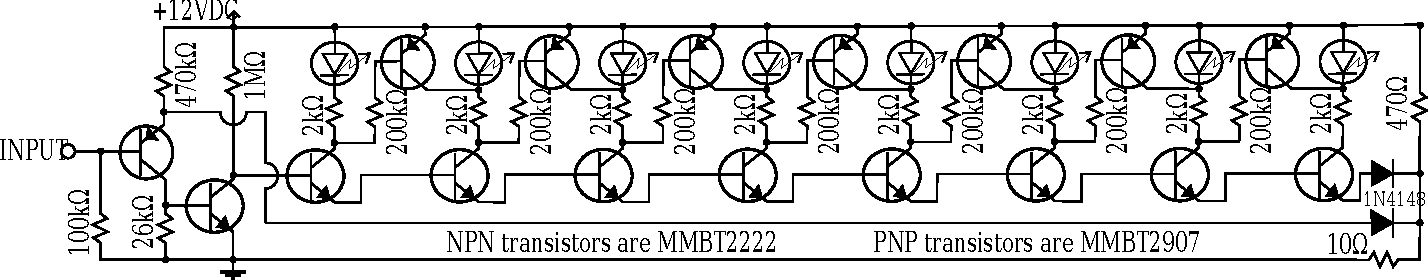
\includegraphics[width=\textwidth]{schematic.pdf}
\caption{\label{fig:frog}Schematic of  novel discrete transistor LED SWIM device.}
\end{figure}
           \begin{floatrow}
             \ffigbox{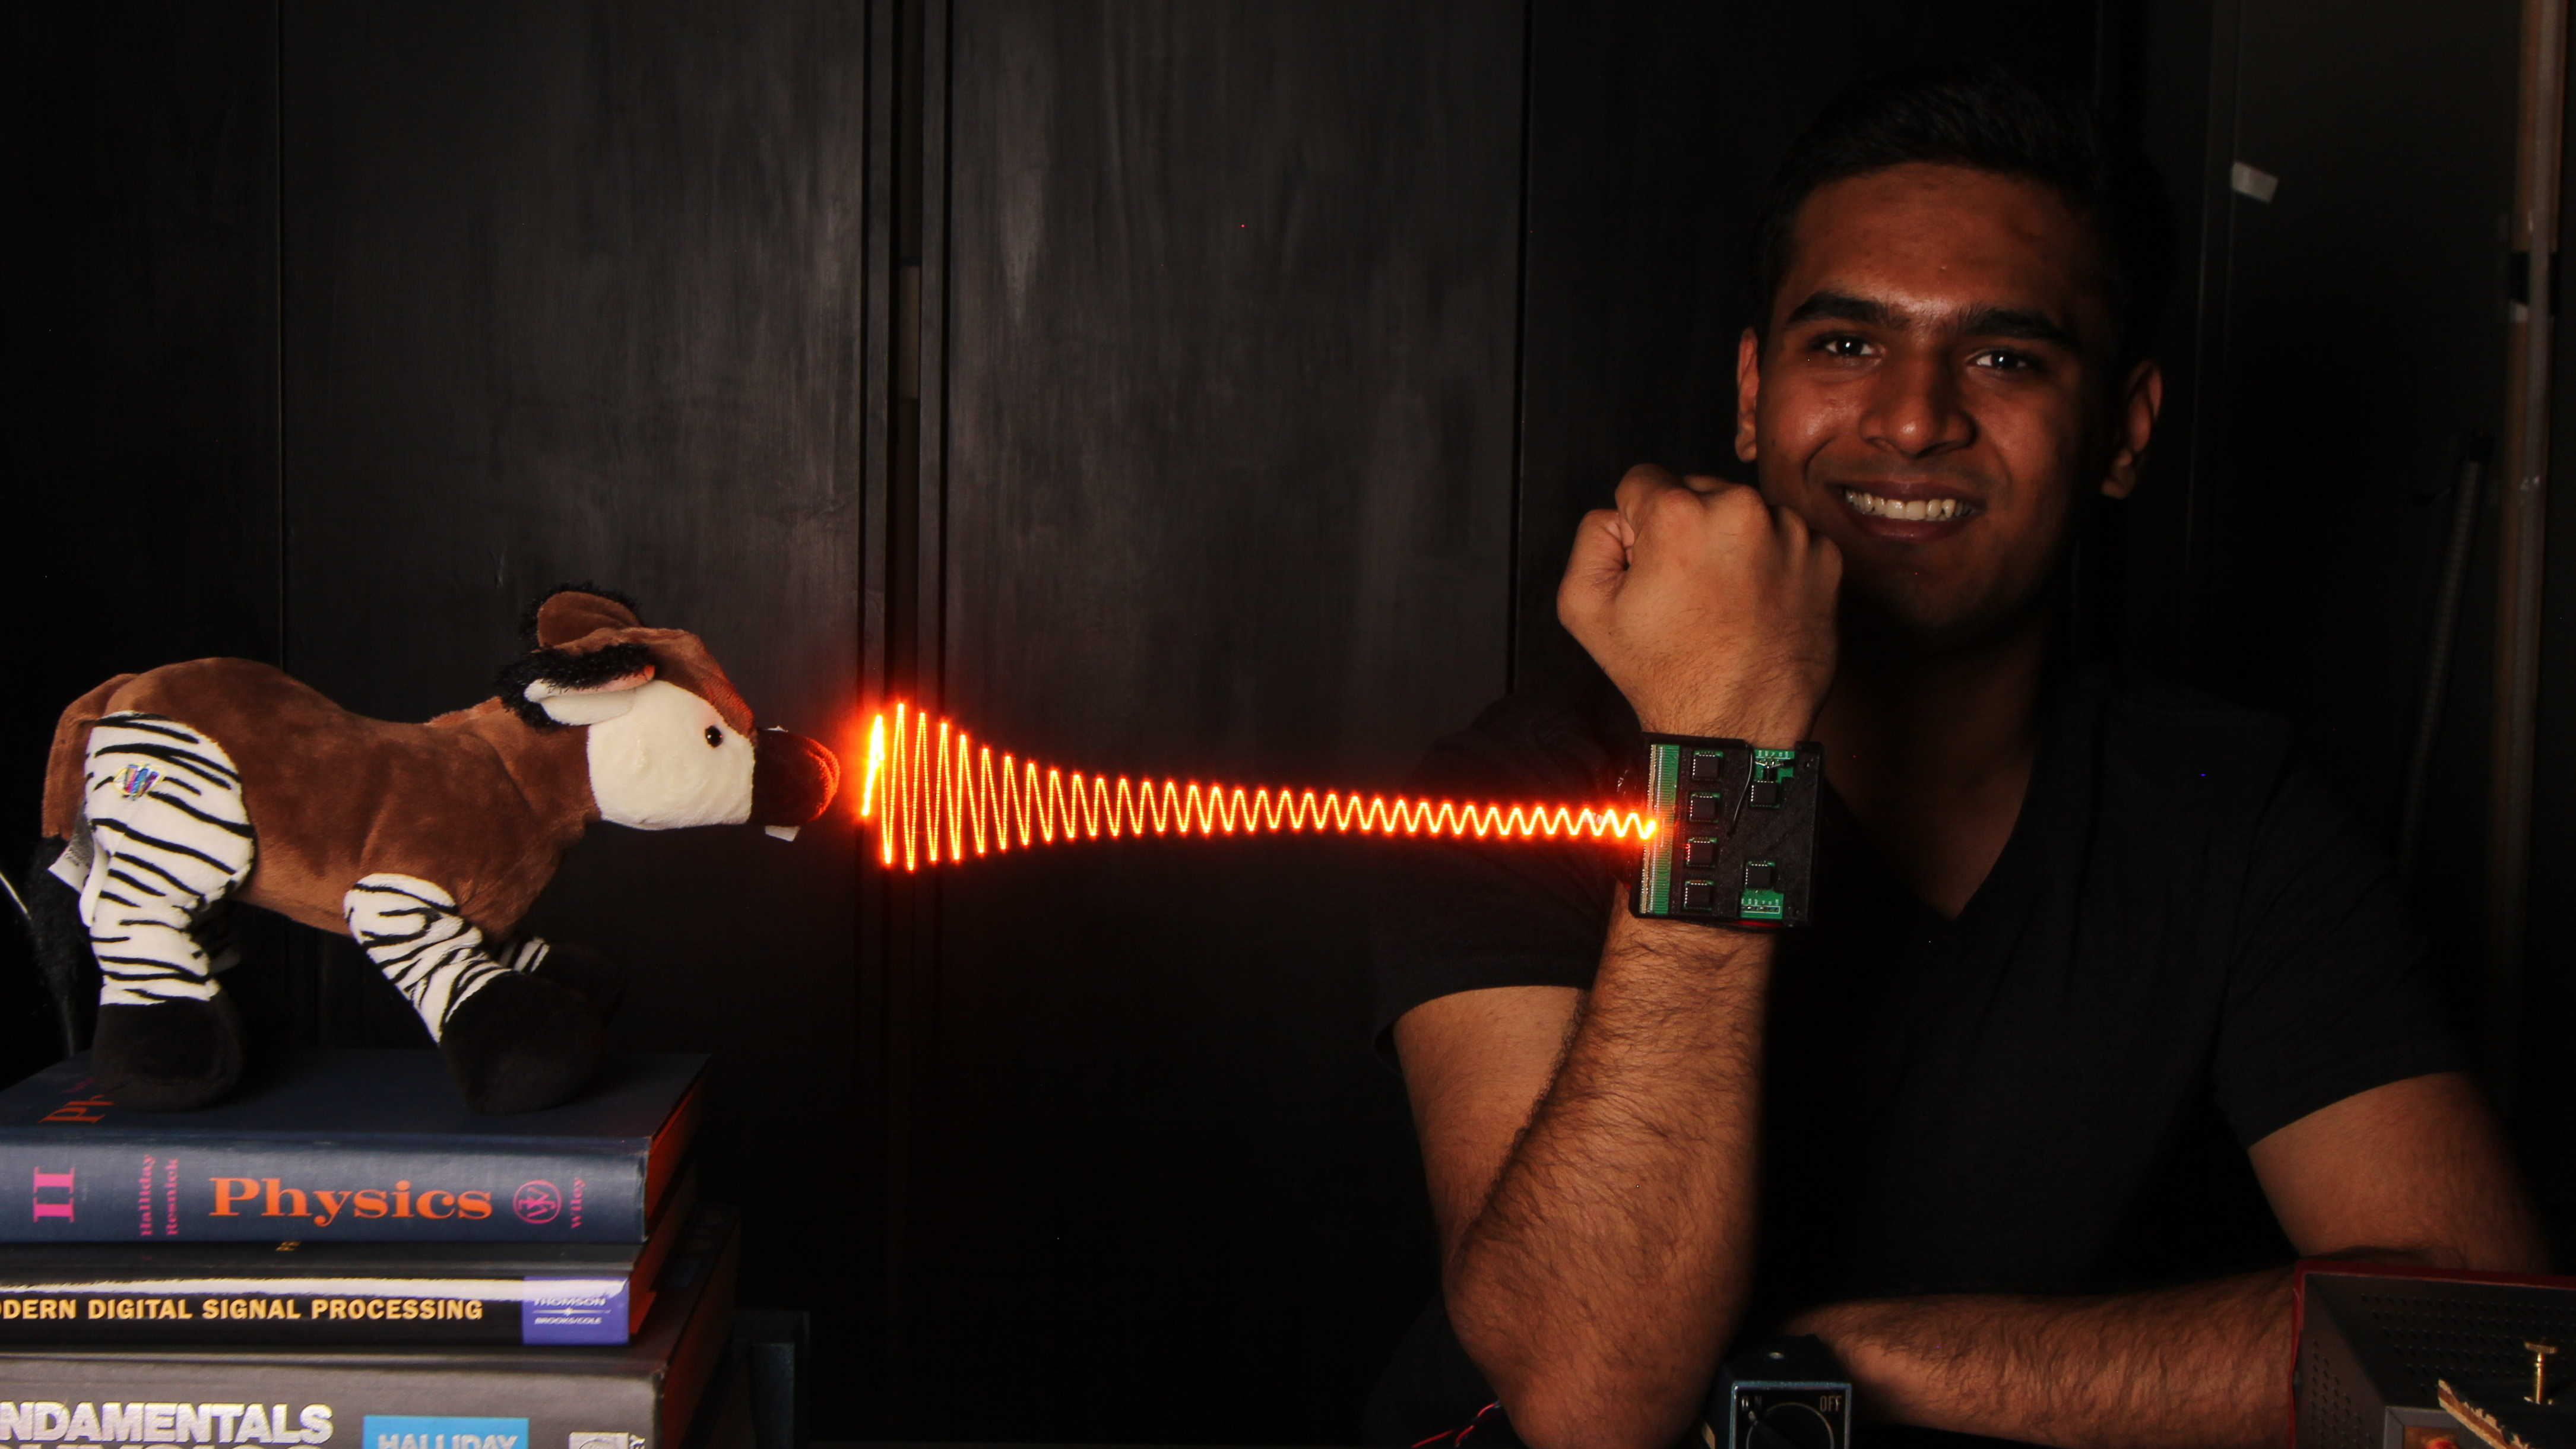
\includegraphics[scale = 0.0371]{sarangs.jpg}}{\caption{}}
 			 \ffigbox{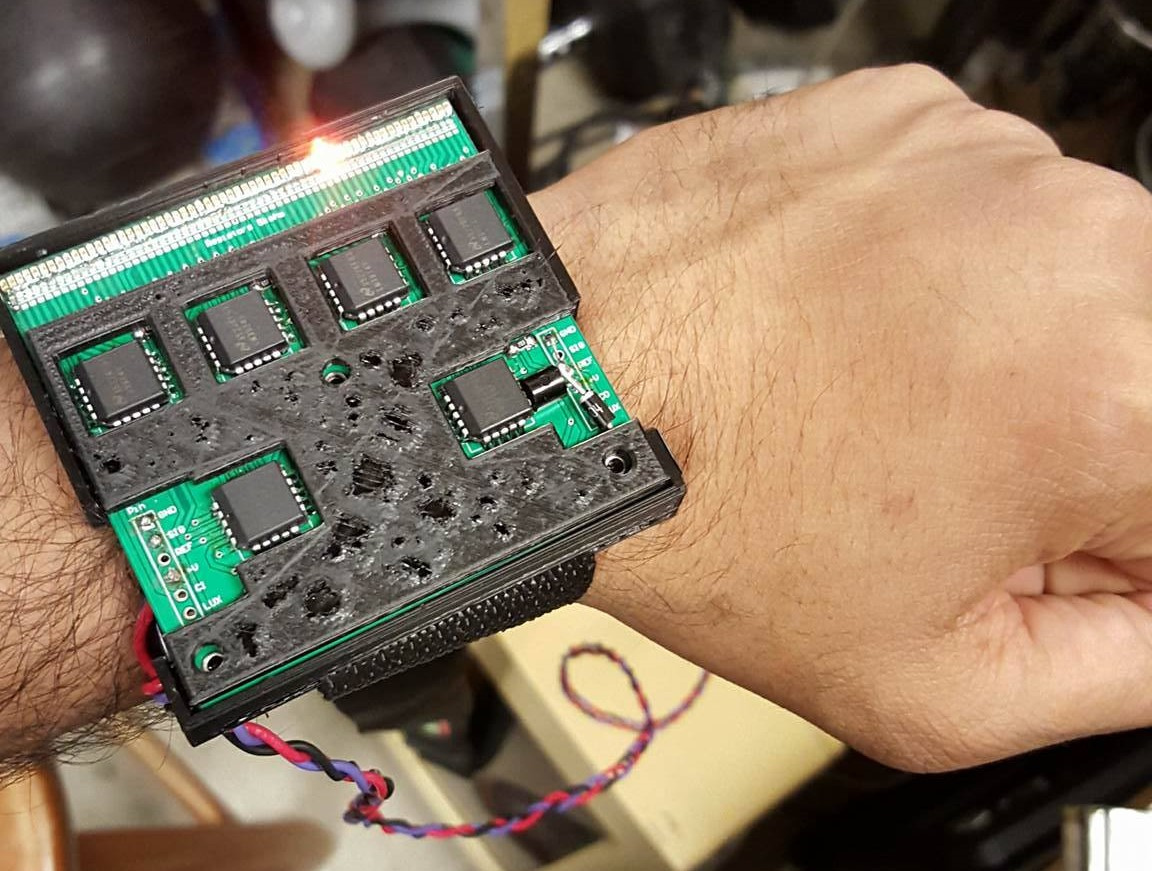
\includegraphics[scale = 0.104]{microswims.jpg}}{\caption{}}
           \end{floatrow}

           \begin{floatrow}
             \ffigbox{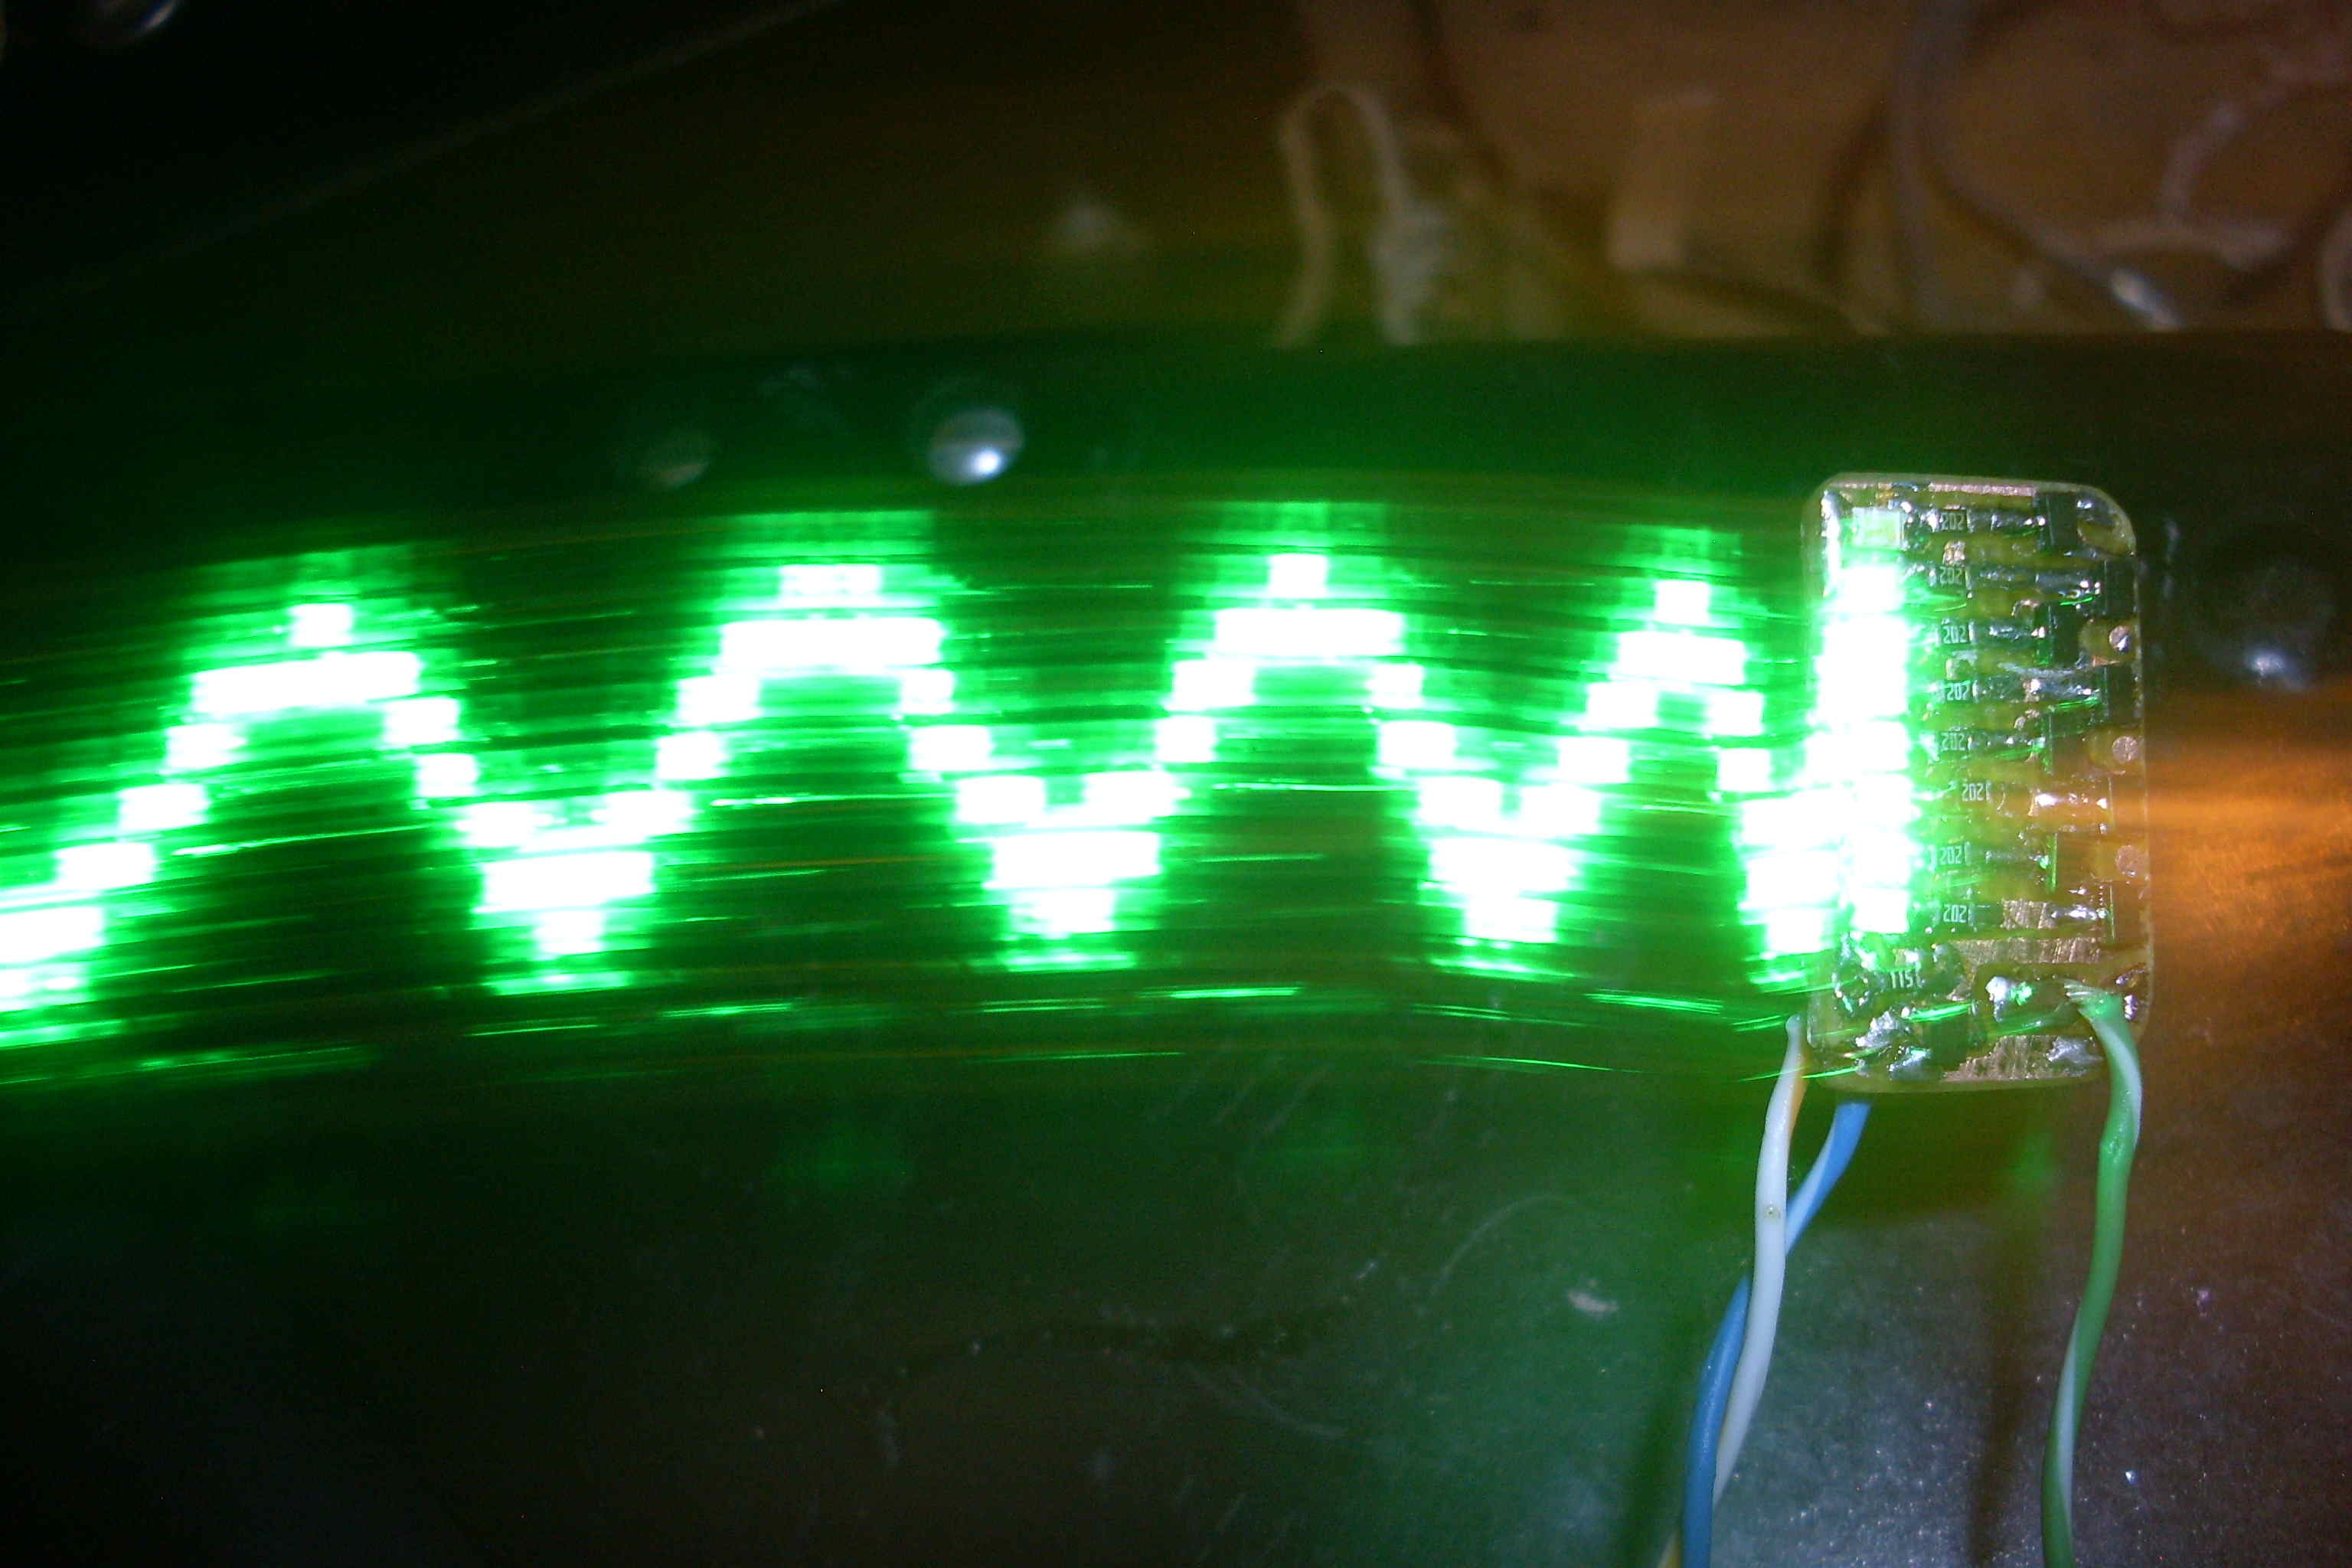
\includegraphics[scale = 0.06215]{SDC11632s.jpg}}{\caption{}}
             \ffigbox{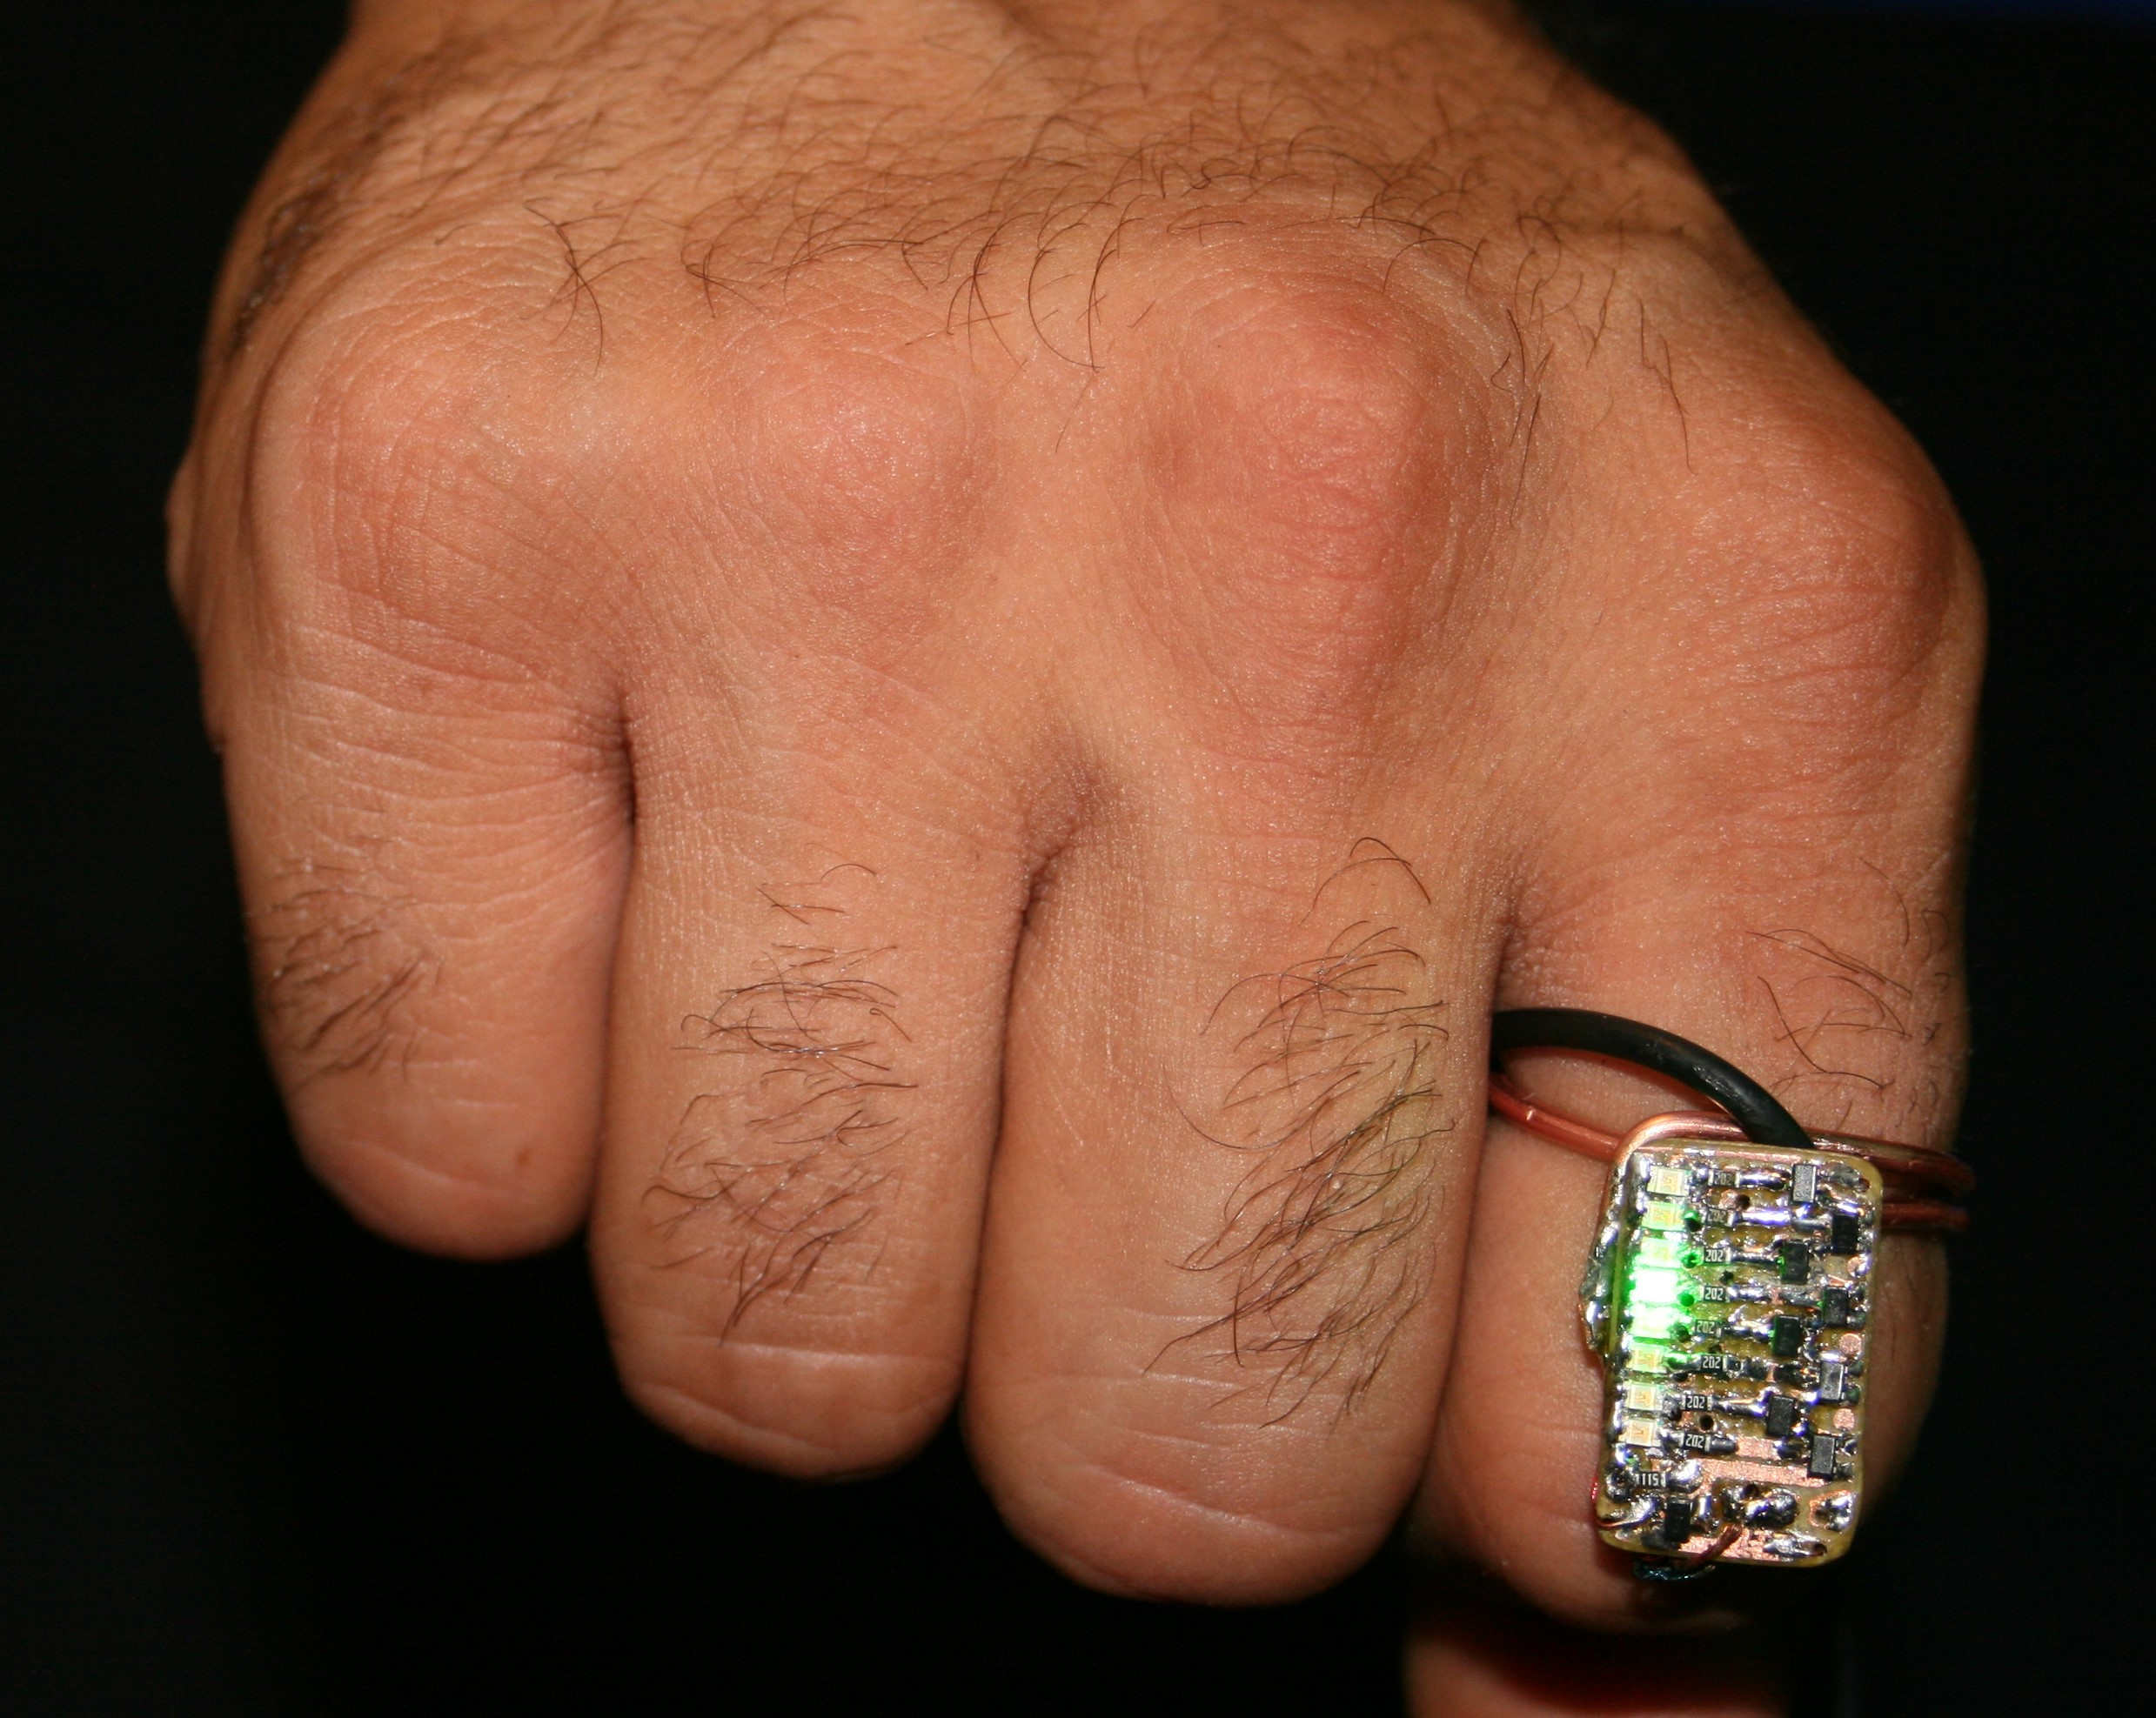
\includegraphics[scale = 0.0484]{SWIMs.jpg}}{\caption{}}
           \end{floatrow}
\section{Recent Advances in SWIM}
Recently new interest has been raised over SWIM, and several have been built.
The first and simplest to implement were digital, with a microcontroller driving cascaded serially programmable WS2812 RGB "neopixels", which can conveniently be purchased in a strip, but pixels are large (greater than 0.5cm) and they suffer from a limited refresh rate. 
Next SWIMs were built around the LM3914 cascadable 10 segment dot/bar graph display driver IC, which produces excellent results with a high degree of accuracy, tested up to at least 100 cascaded ICs for HD pixel counts and large scale size, the modular design used is seen in Fig.1.
The LM3914 was measured to have a bandwidth around 2Mhz, which translates to a very high "refresh rate" and the simple analog system controlling it approaches linear time invariancy, eliminating the possibility of any lag, so the system always responds instantly and the experience is seamless and convincing: humanistic integrity is maintained.\\
LM3914 ICs were used to make a wristworn "microswim" pictured in Fig.4, which is a 60 pixel SWIM, utilizing 0603 size SMD LEDs, which fits on a 6cm square PCB. An image produced with this SWIM is found in Fig.3. 
A novel discrete transistor circuit has been devised, pictured in Fig.2, which makes a low pixel count SWIM smaller and cheaper than is possible with the LM3914. Pictured in Fig.6, an 8 pixel discrete SWIM fits on a 1.25cm by 1.9cm PCB small enough to be worn a ring. An output image from the Ring SWIM is found in Fig. 5.
%
%\section{Visualization of Waves with the Sequential Wave Imprinting Machine}
%One important application of augmediated reality is for making visible the invisible world. It is known that invisible radio %waves are everywhere, permeating all space around us, and thus if these waves are made visible by some means, more may be learned of the world that surrounds us and the way it works. 
%This is the ethos which led Steve Mann to develop the Sequential Wave Imprinting Machine as a teenager in the 1970s. The device was a general purpose analog or digitally controllable linear display of lightbulbs, with which he was able to visually witness (visualize) radio waves in real-time as well as real-space. The device is designed to operated in a simple manner, it is waved about by the user, and as it moves through space, it paints out in light [cite lightpainting? abakographic user interfaces] the radio waves produced by an accompanying radar set.

%When in a dark place or where the ambient light can be controlled to a low level, the system works by the phenomenon of persistance of exposure[cite mann] and makes waves able to be observed with the naked eye by the user as well as onlookers. 

\section{Conclusion}
New wrist and ring worn SWIM devices make the SWIM device more wearable than ever, and LEDs allow high resultion and high luminosity with low power consumption. As a result, clear and bright images are produced in order to visualize waves with phenomenologically augmented reality.

\bibliographystyle{IEEEtran}
% argument is your BibTeX string definitions and bibliography database(s)
%\bibliography{IEEEabrv,../bib/paper}
\bibliography{ref}
%
% <OR> manually copy in the resultant .bbl file
% set second argument of \begin to the number of references
% (used to reserve space for the reference number labels box)
%\begin{thebibliography}{1}

%\bibitem{IEEEhowto:kopka}
%H.~Kopka and P.~W. Daly, \emph{A Guide to \LaTeX}, 3rd~ed.\hskip 1em plus
%  0.5em minus 0.4em\relax Harlow, England: Addison-Wesley, 1999.

%\end{thebibliography}

% that's all folks
\end{document}


